
\chapter{Some Notes on Mathematical Modeling}
These are the steps for mathematical modeling that I have gathered by thinking deep and observing what is happening around me. How my supervisors attack a problem, what is the thought process of professor X in dealing with a problem at one glance, what are the concerns about a specific type of problem (like Stock's problem in PDE theory which is a saddle-node type problem), and what are the main tools to address that problem. These steps in modeling a phenomena mathematically gives me a sense of orientation in a busy world full of new things. This section will be developed overtime, and at some point it can be a chapter of my thesis.

\begin{summary}
	The primary purpose of these notes is to locate the stage of any ongoing project. Also, I will do my best to prepare a kind of checklist for each step that can be used to evaluate the progress of the sub-steps of the project.
\end{summary}

\section{STEP 0: Understanding the phenomena we want to study}

\section{STEP I: Converting Natural Phenomena to a Mathematical Problem }
This step is one of the steps that looks very strange for me. Early from calculus courses and elementary ODE, PDE courses, we can see phrase like ``this Dirichlet boundary condition along with an elliptic PDE models a rod that its two ends are covered with ice at temperature 0'', or ``This saddle-point problem named Stokes problem models a non-compressible fluid''. But they never talk about why this is true, and even how this is possible? Why a bunch of numbers and functions should mimic a very complex phenomena?

There are some very interesting papers written to explain why the mathematics is so effective in modeling the natural world (see \autoref{fig:mathmodelingmatheffectiveness}). In my opinion, this step, although innocent looking, is a totally non-trivial step. Because the nature is what it is, and the fact that some abstract notions and objects can mimic those natural phenomena with nuance details (like the things that happens in bifurcation) is very strange. 

At this step, we need to first \textbf{identify the questions} that we want to answer. This is the most important step that affects all of the subsequence analysis. We need to ask ourselves \textbf{to what level of accuracy} we want our answer? \textbf{To what level of generality} we want our answer be?

This step is the step in which we make our decisions. We decide what details to include or ignore. We decide what are the concrete questions we want to answer. This will determine the right mathematical tools that we can use. 

\begin{summary}[Step I: Converting a natural phenomena to a mathematical problem]
	$ \; $
	\begin{enumerate}[(i)]
		\item The most important thing: What is the question that we want to answer?
		\item We make lots of decisions:
		\begin{itemize}
			\item What is the precision in the answer that we are looking for?
			\item What is the generality that we are after?
			\item What is an appropriate mathematical tool that can be used to model?
		\end{itemize}
		
	\end{enumerate}
\end{summary}

\begin{figure}
	\centering
	\captionsetup{width=.9\linewidth}
	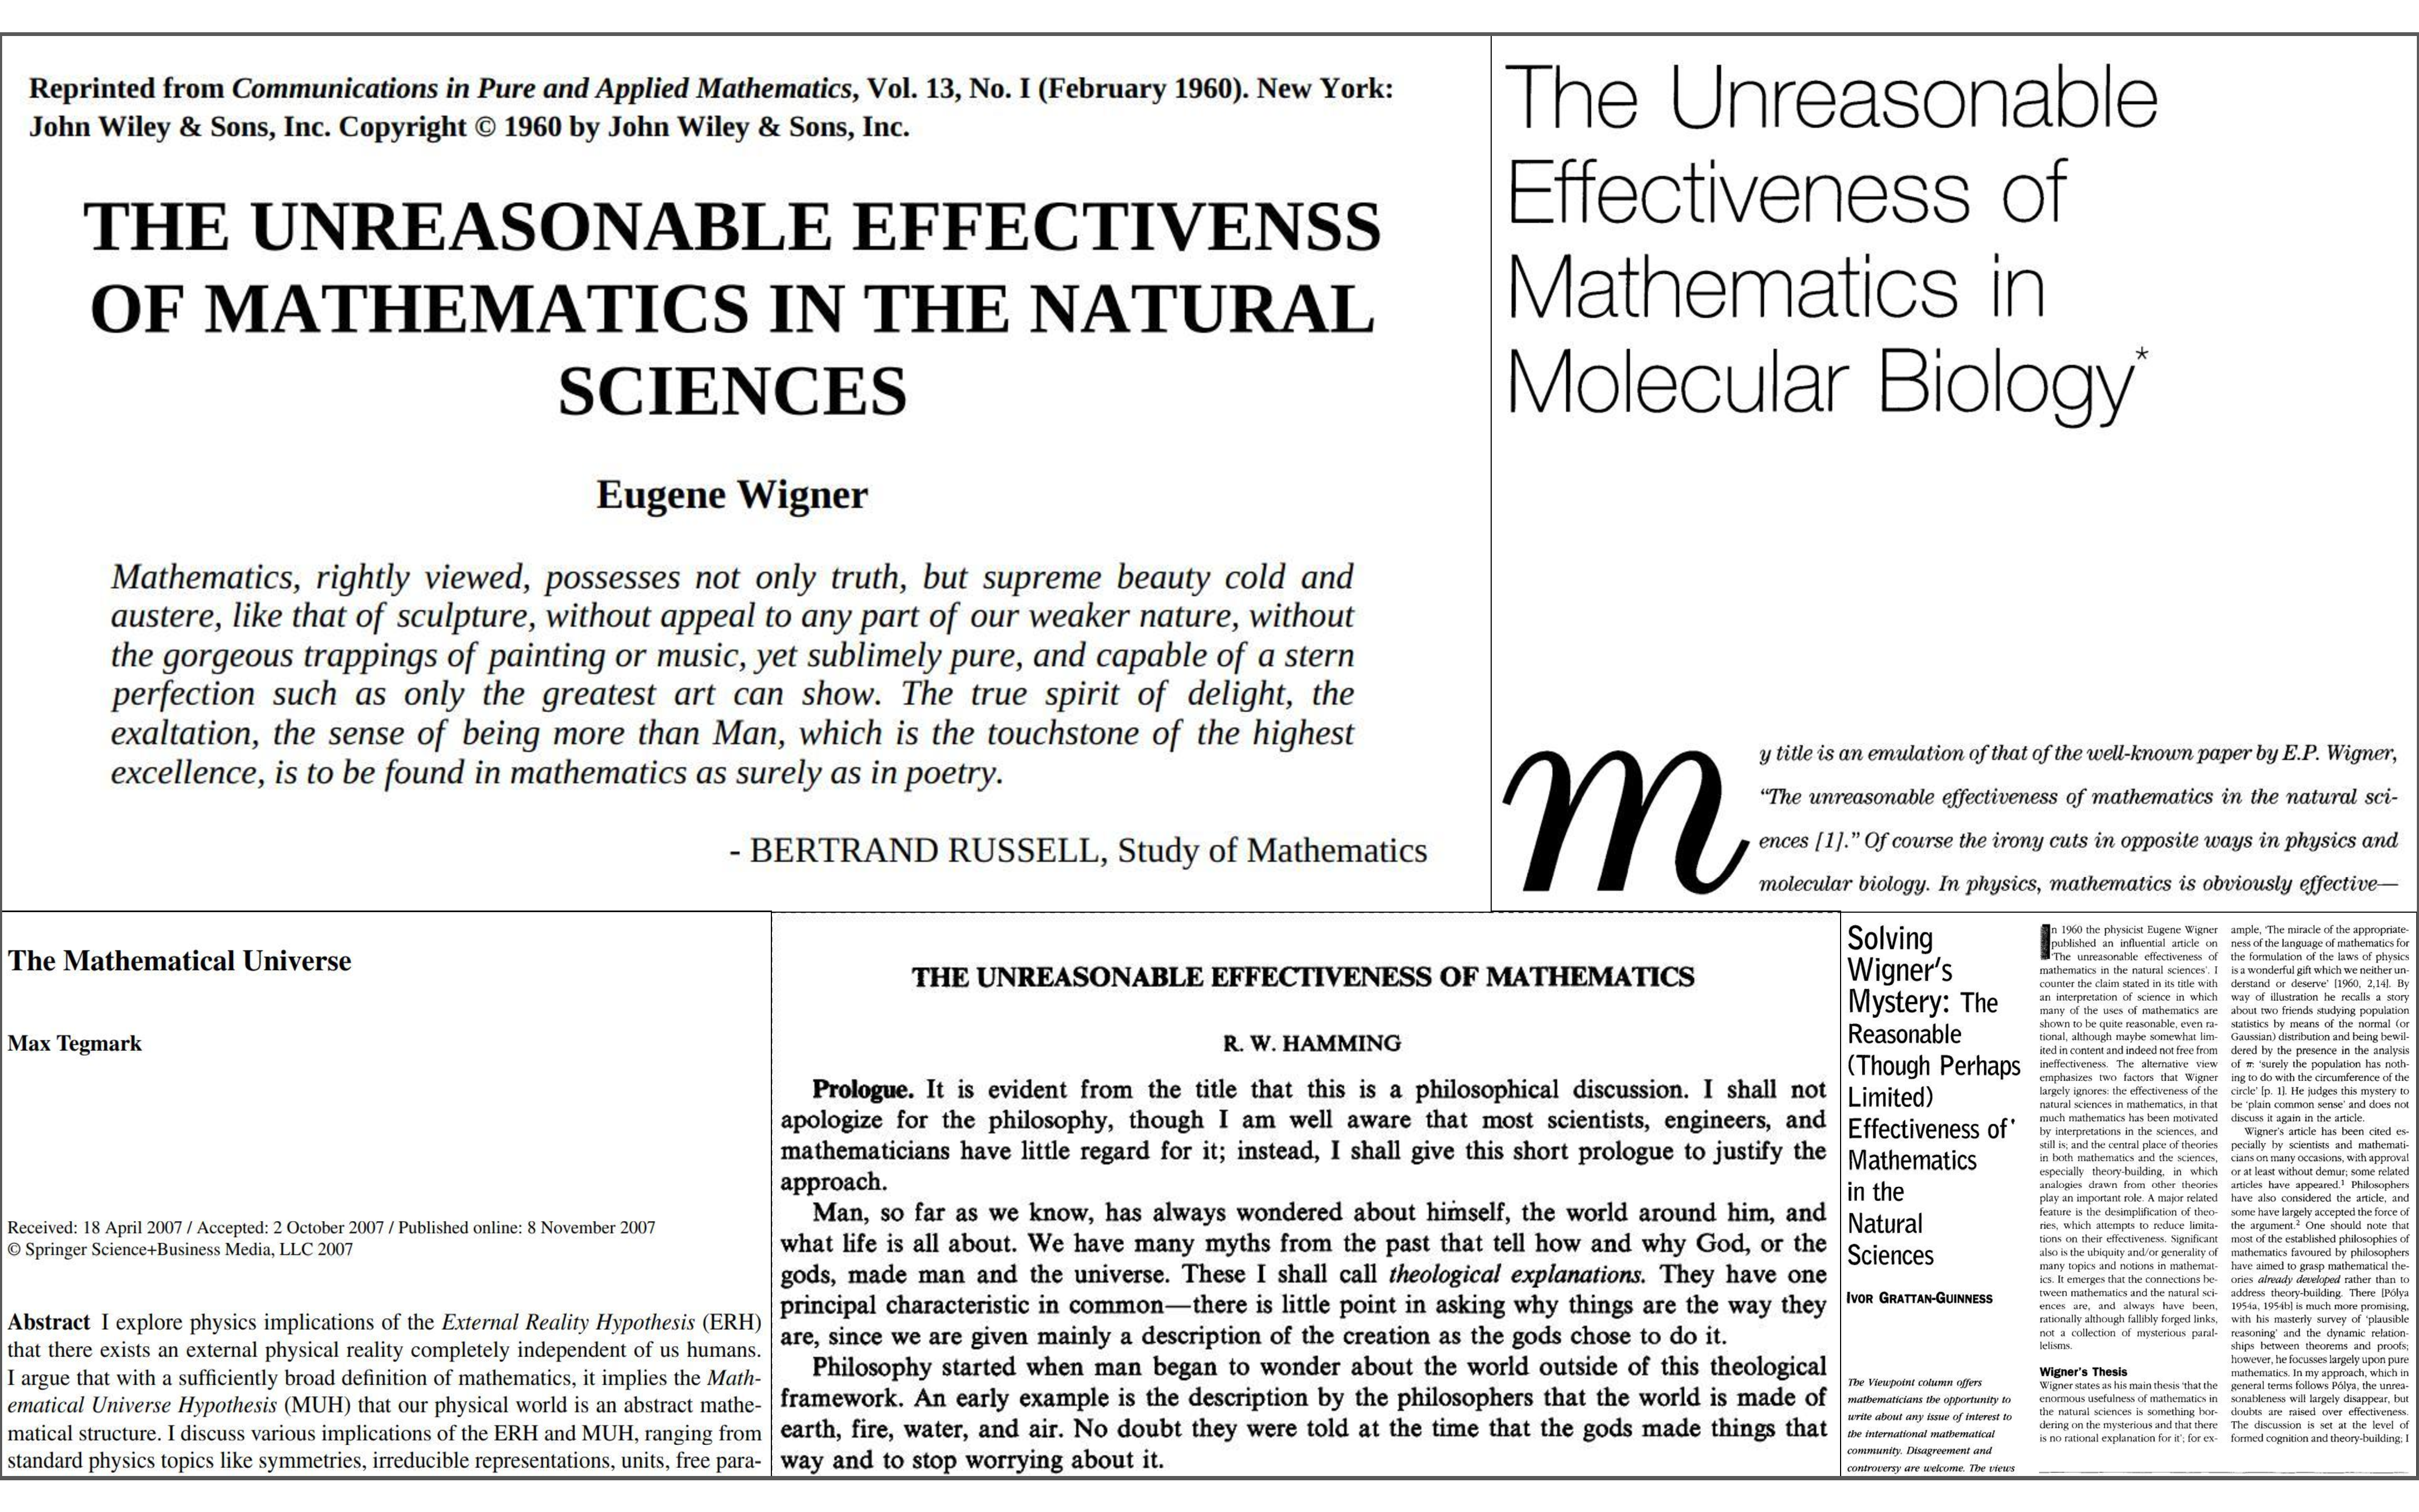
\includegraphics[width=1\linewidth]{images/EffectinvenessOFMath.pdf}
	\caption{A series of papers written after Wigner's famous article published in 1960 \cite{Wigner1995}. Several famous scientists of the time responded to this paper, by expanding the ideas to particular fields, among which are \cite{Hamming1980},  \cite{Lesk2000},  \cite{Tegmark2008}, and \cite{GrattanGuinness2008}. }
	\label{fig:mathmodelingmatheffectiveness}
\end{figure}

\FloatBarrier

\section{STEP II: Mathematical Analysis of the Model in Hand}
After doing the STEP I appropriately, we will have a mathematical description of the phenomena in our hand. This mathematical formulation on the problem can come in my different flavors and forms, We can categorize them by considering their different aspects, like being a discrete or continuous model, being a deterministic or stochastic model, etc. Each of these formulations will have its own appropriate way of treating. So I will discuss their subsequence steps separately.
 
 
\subsection{STEP II: PDE models}
After converting the natural phenomena to a mathematical model containing PDEs, we will have a domain, and a PDE. For instance, let $ \Omega \subset \R^2 $, and we define
\begin{align*}
	-\Delta u  &= g, \qquad \text{on }\Omega, \\
	u &= 0, \qquad \text{on } \partial \Omega.
\end{align*}
In this particular problem, we have a domain, on which we are interested in finding a mapping $ u:\Omega \to \R $ whose partial derivatives satisfies a certain equation. Our first goal is to determine if this problem has a solution (existence), and then to see if the problem as a unique solution (uniqueness), and then to see if the solution is stable (i.e. bounded by the given data). 

\begin{summary}
	Given a PDE in hand, it is important to see if the problem is well-posed (in the sense  of Hadamard). I.e.
	\begin{itemize}[noitemsep]
		\item a solution exists,
		\item the solution is unique, and
		\item the solution is stable.
		
	\end{itemize}
\end{summary}

\subsubsection{Different Formulations of the Problem: Strong vs. Weak Formulation}
To find the answers to these questions, we can formulate our problem in different ways, i.e. strong formulation, or a weak formulation. In the weak formation, we have more relaxed requirements on the solutions. For instance, for a classic solution to satisfy an elliptic Dirichlet boundary value problem, by definition, it needs to have two derivatives while being zero at the boundary (i.e. $ u \in C_c^2(\Omega) $). However, we can relax this requirement by a kind of axiomatic extension of the set of possible solutions. For instance, we know that all $ C_c^2(\Omega) $ functions has a nice interaction with $ C_c^\infty(\Omega) $ functions through the integration by parts formula.
\[ \int_\Omega \nabla u \nabla v = -\int_\Omega u \nabla v \qquad \forall v \in C_c^\infty (\Omega).  \]
Thus we can use this property as a definition of derivative, and define the notion of the weak derivative. We can use this property to formulate the problem in weak sense. 
\[ \int_\Omega \nabla u \ \nabla v = \int_\Omega g v \qquad \forall v \in H_0^1(\Omega). \]
We can now write the problem in a more abstract form by defining bi-linear forms
\[ a: H_0^1 \times H_0^1 \to \R, \qquad l:H_0^1 \to \R \] 
and define 
\[ a(u,v) = \int_\Omega \nabla u\  \nabla v, \qquad l(v) = \int_\Omega gv. \]
Thus we can now write the weak formulation as the following abstract equation, i.e. we say $ u $ satisfies the boundary value problem stated above if it satisfies
\begin{align*}
	&a(u,v)  = l(v), \qquad \forall v \in H_0^1,\\
	&u = 0 \quad \text{on}\ \partial \Omega.
\end{align*}

\subsubsection{well-Posedness}
Writing the problem in hand in abstract form, helps us to use other existing mathematical infrastructure to understand if a solution exists, if it is unique, and if it is stable. For instance, writing the elliptic problem in the form of $ a(u,v) = l(v) $ allows us to use the infrastructure developed in functional analysis to find the answers to our questions. For instance, in this particular case, we can use the Lax-Milgram theorem (which is a kind of generalization to the Ritz-representation theorem) to show that under certain conditions (i.e. the bi-linear form $ a $ being coercive and bounded, and the linear form $ l $ being bounded. ) a solution exists, and is unique and stable (i.e. bounded by the data). Or in the case of the Stokes problem for the non-compressible fluid, we have the  Ladyzhenskaya-Babuška-Brezzi condition (or LBB in short) which is also often called inf-sup condition, is a set of conditions under which the Stokes problem as a unique solution that is stable. 

\begin{summary}[Importance of formulating the mathematical problem appropriately]
	Formulating a mathematical problem in an appropriate way is very crucial. Appropriate formulations allows us to use the existing important theorems in a specific field of mathematics to our advantage. For instance, by formulating a PDE in weak form and using suitable forms, we can use
	\begin{itemize}
		\item Lax-Milgram theorem (generalized form of Ritz-representation theorem) to show the well-posedness of an elliptic problem under certain conditions.
		\item Ladyzhenskaya-Babuška-Brezzi theorem (or LBB in short) to show the well-posedness of the Stokes problem for non compressible fluid.
	\end{itemize}
\end{summary}


\subsubsection{What kind of solutions do we need?}
The well-posedness of a problem is a hunting license to find the actual solutions. Again, we need to revisits our main question in step I. What are we looking for? Is having a solutions in closed form necessary? Can having the solution in a series form (with a high or low convergence rate) enough? Can we get the answers to our question by some sort of qualitative analysis? Is a numerical solution necessary? \textbf{The exact answer to these questions depends on the questions that we want to answer with mathematical modeling.}

\begin{summary}[Solutions to the PDE]
	After getting the hunting license and being sure about the well-posedness of the problem, we need to revisit our original question to decide what we want to do with the solution? The solution can be found in many ways that might be suitable for some cases and and overkill for other cases.
	\begin{itemize}
		\item closed form solution
		\item series solution (with poor or good convergence rate)
		\item some contracting map 
		\item local solution (for local behaviour analysis)
		\item numerical solution
		\item etc.
	\end{itemize}
\end{summary}

\subsubsection{Numerical Solution}
After deciding on if we need a numerical solution, we can use different approaches, each of which has its own treatment. Here I will only talk about the finite element methods. In the finite element method, we find a suitable finite dimensional sub-space of the solution space ($ H_0^1 $ in the case of the elliptic Dirichlet problem) and formulate the problem in discrete form. For instance, if we can generate a triangulation of a domain $ \Omega $ and define some local basis functions e.g. some continouse and piece-wise affine functions that each of them is non-zero only at one node. Thus we can express our function in the weak formulation in this form
\[ u = \sum_{i=1}^{n}U_i \phi_i(x), \qquad g = \sum_{i=1}^{n}G_i \phi_i(x). \]
By substituting this in the weak formulation, we will get the following system of linear equations
\[ A U = G, \]
where the matrix $ A $ (stiffness matrix) and the vector $  G $ are the given data and we want to find the vector $ U $. Or in the case of the Stokes problem, we will get the following system of equations.
\begin{align*}
	&AU + BP = F, \\
	&B^T U = 0.
\end{align*}
\textbf{Note}: After projecting the problem to a finite dimensional sub-space, it is not necessarily true the the well-posedness of the problem in the infinite dimensional Hilbert space carries over to the finite dimensional sub-space. For instance, in the case of the Stokes problem, the well-posedness does not carry over and we need to study the well-posedness of the discrete problem.

\subsubsection{Error Estimate}
Projecting an infinite dimensional space to a finite dimensional space introduces some errors that we need to be sure we can quantify and understand how does that error scales with the mesh size (i.e. the dimension of the finite dimensional sub-space).



\section{What Is the Flux, Really?}
Here in this section we will go deeper into the notion of flux in particle transport which is the central part mathematical modeling of living systems. I will try to connect this notion with mathematical objects with clear definitions rather than providing vague intuition.

Generally speaking, flux is a surface integral of some vector field, and by designing that vector field accurately, we can use the notion of flux in different contexts. Here we will design the notion of flux to study particles and their densities assuming they are non-compressible fluids. Let $ \Omega \subset \R^3 $. Define 
\[ J = \rho v \]
where
\[ \rho: \Omega\times \R \to \R, \qquad v:\Omega\times \R\to\R^3, \]
representing the density and the velocity of the scalar field respectively. But what is the velocity of $ \rho $? Here is the part where the notion of volume preserving diffeomorphisms become useful. Let $ X_0 \in\Omega $ denote the position of a point particle in the domain. Then its trajectory over time is determined by the action of the group $ \set{g^t}_{t \in T} $ on $ X_0 $. For instance $ X(t) = g^t X_0 $. Since we have assumed that the species are in form of non-compressible fluids, then the group $ \set{g^t} $ is a subgroup of the group of all diffeomorphisms that preserves the volume. For a fixed $ X_0 \in \Omega $ its orbit is defined to be
\[ \operatorname{Orbit}(X_0) = \set{g^t X_0 \ |\ t \in T}. \]
At any time $ t $, $ v(X,t) $ is defined to be
\[ v(X,t) = \lim_{\Delta t \to 0} \frac{g^{t+\Delta t} X - g^{t} X}{\Delta t} \]
This means that for $ X_0 \in A $ we can write
\[ g^{\Delta t} X_0 = X_0 + \vec{v}(X_0) \Delta t + O(\Delta t ^2) \]
which means that the effect of $ g^{\Delta t} $ on the point $ X_0 $ just shifting $ X_0 $ in the direction $ \vec{v}(X_0) \Delta t  $. In the figure below we can see this approximation on a particular orbit.
\begin{figure}[h!]
	\centering
	
	
	
	\tikzset{every picture/.style={line width=0.75pt}} %set default line width to 0.75pt        
	
	\begin{tikzpicture}[x=0.75pt,y=0.75pt,yscale=-1,xscale=1]
		%uncomment if require: \path (0,300); %set diagram left start at 0, and has height of 300
		
		%Straight Lines [id:da7253651408536048] 
		\draw [color={rgb, 255:red, 160; green, 160; blue, 160 }  ,draw opacity=1 ][line width=0.75]    (136.83,103.17) -- (149.81,85.61) ;
		\draw [shift={(151,84)}, rotate = 126.47] [color={rgb, 255:red, 160; green, 160; blue, 160 }  ,draw opacity=1 ][line width=0.75]    (6.56,-1.97) .. controls (4.17,-0.84) and (1.99,-0.18) .. (0,0) .. controls (1.99,0.18) and (4.17,0.84) .. (6.56,1.97)   ;
		%Curve Lines [id:da4933662152703622] 
		\draw    (82,133.33) .. controls (151.8,130.12) and (147.11,57.99) .. (164.66,37.97) ;
		\draw [shift={(166.67,36)}, rotate = 140.19] [fill={rgb, 255:red, 0; green, 0; blue, 0 }  ][line width=0.08]  [draw opacity=0] (7.14,-3.43) -- (0,0) -- (7.14,3.43) -- (4.74,0) -- cycle    ;
		%Curve Lines [id:da8486116401578401] 
		\draw    (164,38.33) .. controls (173,29.67) and (176.33,28.67) .. (188,22.33) ;
		%Shape: Circle [id:dp6250392978342221] 
		\draw  [fill={rgb, 255:red, 0; green, 0; blue, 0 }  ,fill opacity=1 ] (135,103.17) .. controls (135,102.15) and (135.82,101.33) .. (136.83,101.33) .. controls (137.85,101.33) and (138.67,102.15) .. (138.67,103.17) .. controls (138.67,104.18) and (137.85,105) .. (136.83,105) .. controls (135.82,105) and (135,104.18) .. (135,103.17) -- cycle ;
		%Shape: Circle [id:dp5689260707692063] 
		\draw  [fill={rgb, 255:red, 74; green, 144; blue, 226 }  ,fill opacity=1 ] (149.33,70.5) .. controls (149.33,69.49) and (150.15,68.67) .. (151.17,68.67) .. controls (152.18,68.67) and (153,69.49) .. (153,70.5) .. controls (153,71.51) and (152.18,72.33) .. (151.17,72.33) .. controls (150.15,72.33) and (149.33,71.51) .. (149.33,70.5) -- cycle ;
		
		% Text Node
		\draw (134,107.4) node [anchor=north west][inner sep=0.75pt]  [font=\tiny]  {$X_{0}$};
		% Text Node
		\draw (151.67,89.73) node [anchor=north west][inner sep=0.75pt]  [font=\tiny,color={rgb, 255:red, 116; green, 116; blue, 116 }  ,opacity=1 ]  {$\vec{v}( X_{0})$};
		% Text Node
		\draw (156.67,61.4) node [anchor=north west][inner sep=0.75pt]  [font=\tiny,color={rgb, 255:red, 0; green, 61; blue, 133 }  ,opacity=1 ]  {$g^{\Delta t} X_{0} =X_{0} +V( X_{0}) \Delta t+O\left( \Delta t^{2}\right)$};
		
		
	\end{tikzpicture}
\end{figure}
Let $ \sigma $ be any surface given in the domain. We claim that the rate of volume passing through this membrane is given by
\[ \frac{dV}{dt} = \int_\sigma \vec{v}\cdot \hat{n}\ dA. \]
To see this $ \Delta A $ be the area of a flat square tangent to the membrane at point $ X_0 $ on the surface. See the figure below.
\begin{figure}[h!]
	\centering
	
	
	\tikzset{every picture/.style={line width=0.75pt}} %set default line width to 0.75pt        
	
	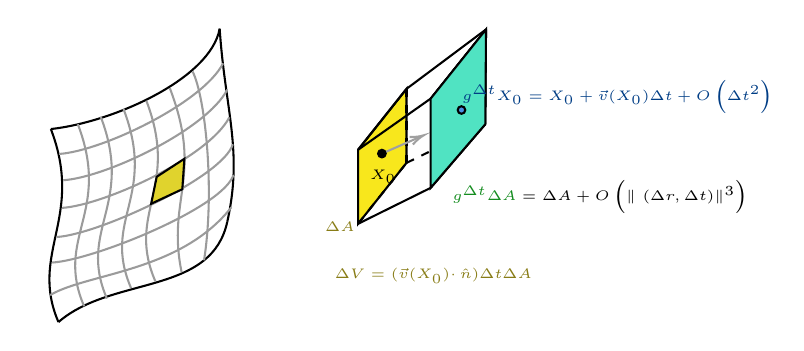
\begin{tikzpicture}[x=0.75pt,y=0.75pt,yscale=-1,xscale=1]
		%uncomment if require: \path (0,300); %set diagram left start at 0, and has height of 300
		
		%Shape: Polygon [id:ds09456144699087154] 
		\draw  [fill={rgb, 255:red, 248; green, 231; blue, 28 }  ,fill opacity=1 ] (178.67,88.67) -- (202,59.33) -- (202,95) -- (178.67,124.33) -- cycle ;
		%Curve Lines [id:da4604489904212945] 
		\draw    (30.67,78.67) .. controls (61,75.33) and (107.67,54.33) .. (112,30.33) ;
		%Curve Lines [id:da6967720169789406] 
		\draw    (34.33,171.67) .. controls (20,138.33) and (47,121.33) .. (30.67,78.67) ;
		%Curve Lines [id:da35266638580627574] 
		\draw    (34.33,171.67) .. controls (54,154.56) and (86.77,156.23) .. (104.47,141.91) .. controls (109.87,137.54) and (113.87,131.68) .. (115.67,123.33) ;
		%Curve Lines [id:da4240338947405422] 
		\draw    (115.67,123.33) .. controls (123.33,89) and (114.67,70) .. (112,30.33) ;
		%Curve Lines [id:da691890187484379] 
		\draw [color={rgb, 255:red, 155; green, 155; blue, 155 }  ,draw opacity=1 ]   (46.67,164) .. controls (32.33,130.67) and (60,119) .. (43.67,76.33) ;
		%Curve Lines [id:da4043207998593765] 
		\draw [color={rgb, 255:red, 155; green, 155; blue, 155 }  ,draw opacity=1 ]   (57.67,160.33) .. controls (43.33,127) and (71,115.33) .. (54.67,72.67) ;
		%Curve Lines [id:da5252238052351152] 
		\draw [color={rgb, 255:red, 155; green, 155; blue, 155 }  ,draw opacity=1 ]   (69.33,155.33) .. controls (55,122) and (82,111.67) .. (65.67,69) ;
		%Curve Lines [id:da31270908120152363] 
		\draw [color={rgb, 255:red, 155; green, 155; blue, 155 }  ,draw opacity=1 ]   (81,152) .. controls (66.67,118.67) and (93,107.67) .. (76.67,65) ;
		%Curve Lines [id:da6303057039241056] 
		\draw [color={rgb, 255:red, 155; green, 155; blue, 155 }  ,draw opacity=1 ]   (93.67,147.67) .. controls (86.33,112) and (104.33,101.67) .. (88,59) ;
		%Curve Lines [id:da8218053838878148] 
		\draw [color={rgb, 255:red, 155; green, 155; blue, 155 }  ,draw opacity=1 ]   (104.47,141.91) .. controls (109.67,109) and (105.33,64) .. (99,51) ;
		%Curve Lines [id:da8308238051916903] 
		\draw [color={rgb, 255:red, 155; green, 155; blue, 155 }  ,draw opacity=1 ]   (113.67,47) .. controls (103.67,66.33) and (55,89.33) .. (34.67,90.67) ;
		%Curve Lines [id:da02053447085552529] 
		\draw [color={rgb, 255:red, 155; green, 155; blue, 155 }  ,draw opacity=1 ]   (115.67,59.67) .. controls (105.67,79) and (57,102) .. (36.67,103.33) ;
		%Curve Lines [id:da5282822241031992] 
		\draw [color={rgb, 255:red, 155; green, 155; blue, 155 }  ,draw opacity=1 ]   (116.67,73) .. controls (106.67,92.33) and (56.33,115.33) .. (36,116.67) ;
		%Curve Lines [id:da23816183015057169] 
		\draw [color={rgb, 255:red, 155; green, 155; blue, 155 }  ,draw opacity=1 ]   (118.33,86) .. controls (113.67,101.67) and (54,129.33) .. (33.67,130.67) ;
		%Curve Lines [id:da569405412784046] 
		\draw [color={rgb, 255:red, 155; green, 155; blue, 155 }  ,draw opacity=1 ]   (118.67,100.67) .. controls (114,116.33) and (51.67,141.67) .. (31.33,143) ;
		%Curve Lines [id:da11295701912713185] 
		\draw [color={rgb, 255:red, 155; green, 155; blue, 155 }  ,draw opacity=1 ]   (117.67,116.33) .. controls (93,147.67) and (48.33,148) .. (30.33,158.67) ;
		%Straight Lines [id:da4575502778776137] 
		\draw    (178.67,88.67) -- (202,59.33) ;
		%Straight Lines [id:da09259804747392031] 
		\draw    (178.67,124.33) -- (178.67,88.67) ;
		%Straight Lines [id:da5208713033396146] 
		\draw  [dash pattern={on 3pt off 3pt}]  (202,95) -- (202,59.33) ;
		%Straight Lines [id:da5610562629835913] 
		\draw  [dash pattern={on 3pt off 3pt}]  (178.67,124.33) -- (202,95) ;
		%Straight Lines [id:da25649545572729315] 
		\draw [color={rgb, 255:red, 160; green, 160; blue, 160 }  ,draw opacity=1 ][line width=0.75]    (190.17,90.5) -- (208.5,82.47) ;
		\draw [shift={(210.33,81.67)}, rotate = 156.35] [color={rgb, 255:red, 160; green, 160; blue, 160 }  ,draw opacity=1 ][line width=0.75]    (6.56,-1.97) .. controls (4.17,-0.84) and (1.99,-0.18) .. (0,0) .. controls (1.99,0.18) and (4.17,0.84) .. (6.56,1.97)   ;
		%Shape: Circle [id:dp4347516737268753] 
		\draw  [fill={rgb, 255:red, 0; green, 0; blue, 0 }  ,fill opacity=1 ] (188.33,90.5) .. controls (188.33,89.49) and (189.15,88.67) .. (190.17,88.67) .. controls (191.18,88.67) and (192,89.49) .. (192,90.5) .. controls (192,91.51) and (191.18,92.33) .. (190.17,92.33) .. controls (189.15,92.33) and (188.33,91.51) .. (188.33,90.5) -- cycle ;
		%Straight Lines [id:da9970436041671149] 
		\draw    (213.67,64) -- (240.33,30.67) ;
		%Straight Lines [id:da342511901706108] 
		\draw    (213.67,107) -- (213.67,64) ;
		%Straight Lines [id:da5902552900557785] 
		\draw    (240,76.33) -- (240.33,30.67) ;
		%Straight Lines [id:da8931061197488246] 
		\draw    (213.67,107) -- (240,76.33) ;
		%Straight Lines [id:da6468976920553455] 
		\draw    (178.67,124.33) -- (213.67,107) ;
		%Straight Lines [id:da7362591464280432] 
		\draw    (178.67,88.67) -- (213.67,64) ;
		%Straight Lines [id:da5565256227844282] 
		\draw    (202,59.33) -- (240.33,30.67) ;
		%Straight Lines [id:da34026137798256473] 
		\draw  [dash pattern={on 3pt off 3pt}]  (202,95) -- (240,76.33) ;
		%Shape: Polygon [id:ds9396511578559401] 
		\draw  [fill={rgb, 255:red, 80; green, 227; blue, 194 }  ,fill opacity=1 ] (240.33,30.67) -- (240,76.33) -- (235.75,81.28) -- (213.67,107) -- (213.67,64) -- cycle ;
		%Shape: Circle [id:dp5366643183971873] 
		\draw  [fill={rgb, 255:red, 74; green, 144; blue, 226 }  ,fill opacity=1 ] (226.67,69.5) .. controls (226.67,68.49) and (227.49,67.67) .. (228.5,67.67) .. controls (229.51,67.67) and (230.33,68.49) .. (230.33,69.5) .. controls (230.33,70.51) and (229.51,71.33) .. (228.5,71.33) .. controls (227.49,71.33) and (226.67,70.51) .. (226.67,69.5) -- cycle ;
		%Shape: Polygon [id:ds3478569100900799] 
		\draw  [fill={rgb, 255:red, 224; green, 211; blue, 45 }  ,fill opacity=1 ] (95,93) -- (94,107.67) -- (79,114.67) -- (81.67,101.67) -- cycle ;
		
		% Text Node
		\draw (183,96.73) node [anchor=north west][inner sep=0.75pt]  [font=\tiny]  {$X_{0}$};
		% Text Node
		\draw (227.33,53.73) node [anchor=north west][inner sep=0.75pt]  [font=\tiny,color={rgb, 255:red, 0; green, 61; blue, 133 }  ,opacity=1 ]  {$g^{\Delta t} X_{0} =X_{0} +\vec{v}( X_{0}) \Delta t+O\left( \Delta t^{2}\right)$};
		% Text Node
		\draw (161.33,122.07) node [anchor=north west][inner sep=0.75pt]  [font=\tiny,color={rgb, 255:red, 136; green, 124; blue, 22 }  ,opacity=1 ]  {$\Delta A$};
		% Text Node
		\draw (222.67,102.07) node [anchor=north west][inner sep=0.75pt]  [font=\tiny]  {$\textcolor[rgb]{0.08,0.55,0.12}{g^{\Delta t} \Delta A} =\Delta A+O\left( \| \ ( \Delta r,\Delta t) \| ^{3}\right)$};
		% Text Node
		\draw (166,144.4) node [anchor=north west][inner sep=0.75pt]  [font=\tiny,color={rgb, 255:red, 136; green, 124; blue, 22 }  ,opacity=1 ]  {$\Delta V=(\vec{v}( X_{0}) \cdotp \hat{n}) \Delta t\Delta A$};
		
		
	\end{tikzpicture}
\end{figure}

\noindent We observe that the point $ X_0 $ moves to $ X_0 + \vec{v}(X_0)\Delta t + \O(\Delta t^2) $. Also, observe that the area any point on $ \Delta A $ distance $ \Delta r $ away from $ X_0 $ will be transferred to 
\[ g^{\Delta t} (X_0 + \Delta r) = X_0 + \Delta r + \vec{v}(X_0 + \Delta r)\Delta t + O(\Delta t^2) = (X_0 + \Delta r) + \vec{v}(X_0) \Delta t + O(\Delta t^2 + \Delta t \Delta r).  \]
Thus the area of the green surface in the figure above will be the same as $ \Delta A $ up to order
$ O((\Delta t^2 + \Delta t \Delta r)^2) $. Note that by the action of $ g^{\Delta t} $, everything in between the yellow and green surfaces will move through the green surface. So the volume that will pass through the green surface is
\[ \Delta V = (\vec{v}(X_0)\Delta t)\cdot \hat{n} \Delta A + O(\Delta t^2) \]
Given that the density of species is $ u $, then the number species passed through the green membrane after time $ \Delta t $ will be
\[ \frac{\Delta N}{\Delta t} = \vec{v}(X_0)\cdot \hat{n}\Delta A + O(\Delta t^2 + \Delta A^2) \]
I.e. we can write
\[ \frac{d N }{dt} = \int_\sigma \vec{v}\cdot \hat{n}\ dA \]


\begin{summary}
	In a nutshell, If we define 
	\[  J = \rho v \]
	where $ \rho :\Omega \times \R \to \R $ is a function representing the density, and $ v: \Omega \times \R \to \R^3 $ is the tangent vector to the orbit of particles generated by the action of group of diffeomorphisms that preserve the volume element $ \set{g^t}_{t\in T} $, then, for any surface $ \sigma \subset \Omega $, the rate of particles passing through the membrane will be
	\[ \frac{dN}{dt} = \int_\sigma J\cdot \hat{n}\ dA. \]
	Then by assuming that no particles will by destroyed to the thin air, and also no particles will born out of blue sky, then we can derive the continuity equation. In any volume $ V $ of our domain enclosed by the surface $ \sigma $, we can write
	\[ \frac{d}{dt} \int_V \rho\ dV = - \int_\sigma J\cdot \hat{n}\ dA = - \int_V \nabla\cdot J dV. \]
	By dropping the integration signs we will get
	\[ \frac{d\rho}{dt} + \nabla\cdot J = 0.  \]
\end{summary}